\documentclass[a4paper]{article}
\usepackage[english]{babel}
\usepackage{pdfpages, titling}
\usepackage{array, float}
\usepackage{cite, tablefootnote}
\usepackage{graphicx, caption, subfigure, wrapfig}
\usepackage{listings}
\usepackage{color}
\usepackage{mathtools, braket}
\usepackage{amssymb}
\usepackage[nottoc]{tocbibind} % references in the toc
\usepackage{textcomp}
\usepackage{minted} % code formatting
\usepackage[hidelinks]{hyperref}
\graphicspath{{Pictures/}} % Specifies the directory where pictures are stored

\newcommand{\vect}[1]{\boldsymbol{#1}}
\newcommand{\subtitle}[1]{%
  \posttitle{%
    \par\end{center}
    \begin{center}\large#1\end{center}
    \vskip0.5em}%
}
\lstset{frame=tb,
  language=Java,
  aboveskip=3mm,
  belowskip=3mm,
  showstringspaces=false,
  columns=flexible,
  basicstyle={\small\ttfamily},
  numbers=none,
  breaklines=true,
  breakatwhitespace=true,
  tabsize=3
}

\author{Jaro Camphuijsen (6042473) and Rahiel Kasim (10447539)}
\date{6 November 2015}
\title{Sunsistemo}
\subtitle{Visualizing the Few Body Problem}
\begin{document}
\maketitle

\tableofcontents

\section*{Abstract}
The physics governing gravity between all bodies of mass in the universe is elegantly expressed by
Newton in a single vector equation. However general analytic solutions are only available for
systems with up to two bodies. In this paper we discuss the physics and algorithms required to build
a numerical simulation of gravity for an arbitrary number of bodies. In addition we look at how to
make a visualization of the few body simulator that is appealing to a large audience. We conclude by
validating the simulation against observations of the Solar System by NASA.

\newpage
\section{Introduction}
% Background, overview of relevant literature, structure of remainder of the report

% Introduce the problem that you have studied
% –Describe what others have done (related work)
% –Describe the structure of your report
% •Make sure that you include enough and appropriate references.
% –Explain for each referenced paper why it is relevant for your paper.
% •In some cases, depending on the size of each part, the problem statement and the related work should be made into separate sections or chapters.

All interactions of gravity are described by Newton's law of universal gravitation. Given initial
positions and velocities, there exists a unique solution for the dynamics of the gravitating bodies.
Analytical solutions are only available for system with at most two bodies. \cite{scholar:nbody}.
For systems with more bodies we have no choice but to resort to numerical methods. Solving this
problem has a long history starting from the father of gravity himself.

When Sir Isaac Newton tried to predict planetary motion around the sun from initial conditions and
some basic geometry he found that over the years his curve deviated from the true motion. He even
correctly blamed this on the multiple interactive gravitational forces exerted by the other bodies
in the system. So the n-body problem was born \cite{wiki:n-body-problem}.

Nowadays n-body simulation is a widely researched and used field. Simulations of galaxies with
billions of stars are used to predict how colliding galaxies will interact with each other. There
are many software libraries available for scientists to conduct these experiments, examples include
AMUSE \cite{amuse}, Pynbody \cite{pynbody} and Nemo \cite{nemo}. These are all sophisticated
interfaces that require knowledge of physics and programming experience. In contrast, our simulation
environment will aim to be accessible and appealing to everyone with an interest in gravity.

This would mean that running a simulation should be as easy as going to a website, clicking on a
button and being in awe of gravity. This can currently only be achieved by programming the
simulation in JavaScript, the only programming language available on the browser. Keeping in mind
that the simulation should work on fast and slower machines, our research will concentrate on the
n-body problem where n is small: the few body problem. To make the simulations appealing it will be
visualized in real-time in 3D.

The remaining structure of this paper is as follows. We start by elucidating the physics in the few
body problem, then we will translate them to usable algorithms with pseudo-code. We continue by
introducing our implementation, Sunsistemo, discuss the visual effects we have implemented to make
it more aesthetically appealing and how we validated the simulation.

% Your report must clearly explain what it is about, and should not just be a repository of facts.
% •The structure of this part depends on the nature of your work. E.g.:
% –Start by describing your methods and algorithms
% •Use formulae, pseudo-code
% –Describe the implementation
% •Describe import choices, leave out what should be self-evident
% •But (well documented) source code goes to appendices, if to be included at all
% –Describe your experiment and the results
% –Interpret your results
% •As with the introduction, the core may be split into separate sections, like methods,
% experimentation and interpretation of the results.

\section{Physics}
In 1687 Sir Isaac Newton published not only his famous three laws of motion, but also his law of
universal gravitation in his book \textit{Philosophiae Naturalis Principia Mathematica}, a treatise
that is regarded as the most important work in the history of science. \cite{wiki:principia} His law
of universal gravitation quantifies the interaction between all particles with mass in the universe,
so it explains not only how objects fall on Earth, but also how the planets in the solar system fall
around the Sun. This law will be at the heart of our simulation.

\subsection{Gravitation}
In vector notation Newton's law of universal gravitation is written as follows:
\begin{equation} \label{eq:newton}
  \vect{F}_{12}=-G\frac{m_{1}m_{2}}{|\vect{r}_{21}|^{2}}\hat{\vect{r}}_{21}
\end{equation}
where $\vec{F}_{12}$ is the vector force on particle 1 (with mass $m_{1}$) exerted by particle 2
(with mass $m_{2}$), $G$ is the gravitational constant, $\vect{r}_{21}$ is the vector pointing from
particle 2 to particle 1 and $\hat{\vect{r}}_{21}$ is its unit vector. \cite{giancoli}

For systems with more than two particles the total force on particle number 1 is:
\begin{equation} \label{eq:multi}
\vect{F}_{1}=\vect{F}_{12} + \vect{F}_{13} + ... + \vect{F}_{1n} = \sum_{i=2}^{n} \vect{F}_{1i}.
\end{equation}

Using Newton's second law, $\vect{F_{1}}=m_{1} \vect{a_{1}}$ and equation \ref{eq:newton} we can
derive an expression for the acceleration on particle 1 due to particle 2:
\begin{align} \label{eq:newton2}
  \vect{F}_{12} &=-G\frac{m_{1}m_{2}}{|\vect{r}_{21}|^{2}}\hat{\vect{r}}_{21} = m_{1} \vect{a_{1}}
  \implies \vect{a_{1}} = -G\frac{m_{2}}{|\vect{r}_{21}|^{2}}\hat{\vect{r}}_{21}
  = G\frac{m_{2}}{|\vect{r}_{12}|^{2}}\hat{\vect{r}}_{12} \nonumber \\[+3mm]
  &= G\frac{m_{2}}{|\vect{r}_{21}|^{3}}\vect{r}_{21}.
\end{align}
Now combining this with equation \ref{eq:multi} we find an expression for the acceleration on
particle 1 due to an arbitrary number of particles:
\begin{equation} \label{eq:nbody}
\vect{a}_{1} = \sum_{i=2}^{n} \vect{a}_{1i} = \sum_{i=2}^{n} G\frac{m_{i}}{|\vect{r}_{i1}|^{3}}\vect{r}_{i1}.
\end{equation}
Given initial conditions for the positions and velocities of the bodies in a system, equation
\ref{eq:nbody} gives the acceleration for a body at any time. In general there is no analytical
solution for the positions of gravitating bodies over time for systems with more than two bodies
\cite{scholar:nbody}. For this reason we have to use numerical methods to calculate the evolution of
the system. How this is done will be discussed in section \ref{sec:numerical} on numerical
integration.

A translation of equation \ref{eq:nbody} to python-esque pseudocode looks like:
\begin{minted}[]{python}
def accel(bodies, i):
    """Calculate acceleration on body i"""
    a = Vector3(0, 0, 0)
    for (j != i) in bodies:
        r = j.position - i.position
        a += G * j.mass / (abs(r) ** 3) * r
    return a
\end{minted}
Note that the acceleration is calculated for all bodies in the system, so we have a nested loop
making this calculation of order $O(n^{2})$.

In the preceding equations the bodies of mass are treated as point particles, i.e. spheres with zero
radius. A more compelling visualization would have bodies with varying radii. To solve the then
emerging problem of bodies being able to move through each other, we will look at the physics of
collisions.

\subsection{Collisions}
\label{sec:collisions}
Bodies with a well determined size can approach each other until their surfaces touch, when this
happens there will be a moment of impact. What happens on such a collision depends on the material
from which the bodies are made. Some options are:
\begin{enumerate}
\item The bodies do not collide but continue their movement. Which is the case for point particles
  with a virtual texture shell.
\item The two colliding bodies merge into one with combined masses. This is a simplification of what
  happens to colliding blobs of fluid with high viscosity.
\item The two bodies collide and change direction based on the initial velocities and body masses.
  This can be a pure elastic collision where energy is conserved before and after the collision, or
  an inelastic collision which does not conserve energy.
\end{enumerate}
For planets and other solid objects the third option makes the most sense, which is the one we will
implement. For a particle of mass $m_1$ and velocity $v_1$ colliding with a particle of mass $m_2$,
the velocity after an elastic collision $v_{1}^*$ is given by:

\begin{equation}
\label{eq:elColl}
 \vect{v}_{1}^*=\vect{v}_{1} - \frac{2 m_2}{m_1 - m_2}\frac{\braket{\vect{v}_{12}|\vect{x}_{12}}}{\| \vect{r}_{12}\|^2}\cdot \vect{r}_{12}
\end{equation}

Where $v_{12} = (v_1 - v_2)$ and $x_{12} = (x_1 - x_2)$, with $v_1, v_2, x_1, x_2$ the velocities
and positions of the particles before the collision took place. Although elastic collisions do not
naturally occur in real world examples of the n-body problem, it was implemented to provide a more
natural interaction between bodies, as before they would just pass through each other. Therefore
when collisions are enabled, at each timestep every body is checked on whether it collides with
another body. In the case of collision, the new velocity is calculated according to equation
\ref{eq:elColl}:

\begin{minted}[]{python}
def collision(bodies, i):
    """Check and calculate collision of body i"""
    for (j != i) in bodies:
        r12 = j.position - i.position
        v12 = j.velocity - i.velocity
        
        if r12 <= (j.radius + i.radius):
            massFactor = 2 * j.mass / (i.mass + j.mass)
            i.v = i.v - r12 * massFactor * (v12 * r12) / abs(r12)^2
\end{minted}

These were the necessary physics for the n-body problem. Given positions we can calculate the
acceleration of the bodies and how they should interact when they collide. How they will actually
move can be computed by numerical integration.

\section{Numerical Integration}
\label{sec:numerical}
Numerical integration is used to evolve the initial positions and velocities of the n-body system
over time. There exist several numerical methods to achieve this. Generally they are used to solve
for solutions of ordinary differential equations. In our case the system to solve is:
\begin{align} \label{eq:ode}
  \frac{d \vect{v}(t)}{dt} &=a(\vect{x}_{1}(t), ..., \vect{x}_{n}(t)) \nonumber \\
  \frac{d \vect{x}(t)}{dt} &= \vect{v}(t),
\end{align}
where the initial conditions $\vect{x}_{i}(0)$ and $\vect{v}_{i}(0)$ are given, and the solution is
the set $(\vect{x}_{1}(t), ..., \vect{x}_{n}(t))$. Here we will review three of such methods to find
these solutions and state which we've chosen to implement and why. Remember that this problem is
three-dimensional and accordingly all the vectors have three dimensions as well.

\subsection{Forward Euler Method}
The simplest of such methods is the so called \textit{Forward Euler Method}. The idea is to take the
initial condition of a variable and to continuously interpolate over a very small timestep $h$ times
the derivative of that variable. These derivatives were defined by system \ref{eq:ode}. Notice that
time is discretized in steps $h$. In general if we denote the \textit{n}th timestep by $t_{n}$ and
the corresponding computed solution as $y_{n}$ the Euler method with initial conditions
$(t_{n}, y_{n})$ is given by:
\begin{equation}
  y_{n+1} = y_n + h f(y_n, t_n),
\end{equation}
where $f$ is the differential equation of the system. \cite{wiki:euler} In our case the computation
for $v_{n+1}$ and $x_{n+1}$ is as depicted in the following pseudocode:
\begin{minted}[]{python}
v[n + 1] = v[n] + h * a[n]
x[n + 1] = x[n] + h * v[n]
\end{minted}
The forward Euler method is simple to implement but has a large error relative to the other methods.
The authors were unable to evolve a system with three bodies using this scheme without them going to
infinity. The local truncation error, or the error in each step of the integrator is proportional to
$h^{2}$ and the global truncation error, the cumulative effect of the local truncation error, is
proportional to $h$. \cite{wiki:euler} Thus the Forward Euler Method is an order 1 integration
method. An alternative way to think about the order of an integrator is as follows: a numerical
integrator of order 5 means that if we shrink the stepsize with a factor of 10, we decrease the
error with a factor of $10^5$.

As a further demonstration we will show how each of the three methods performs on numerically
solving the harmonic oscillator (simple pendulum): $0 = \ddot{x} + \dot{x} = \dot{v} + \dot{x}$,
where $x$ is the position and $v$ the velocity. The performance of the forward Euler method can be
seen in figure \ref{fig:euler}. The integration started from $x_{0}=5$ and $v_{0}=3$ with a stepsize
of $h=0.2$. It is clear that the error of this method is quite large and the pendulum explodes to
infinity. The next method largely improves on this.

\begin{figure}
\center{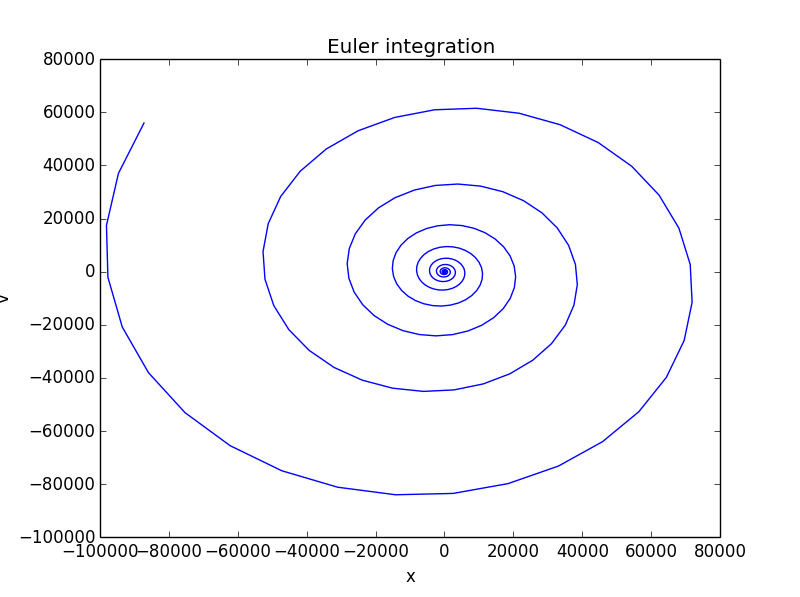
\includegraphics[height=7cm]{Euler_Sling}}
\caption{A solution to the harmonic oscillator numerically integrated with the Forward Euler Method
  starting from $x_{0}=5$ and $v_{0}=3$ with a stepsize of $h=0.2$. We see that the pendulum has an
  unexpected explosive growth in both position and velocity.}
\label{fig:euler}
\end{figure}

\subsection{Symplectic Euler}
A small modification to the forward Euler Method leads to the \textit{Symplectic Euler Method}, the
position is updated using the just calculated new velocity:
\begin{minted}[]{python}
v[n + 1] = v[n] + h * a[n]
x[n + 1] = x[n] + h * v[n + 1]
\end{minted}
A numerical integrator is called \textit{symplectic} if an area of initial conditions in phase space
stays constant under its iteration. What this means physically, is that the energy in the system
stays constant. This difference was immediately apparent in the implementation: it was finally
possible to simulate a stable system of three bodies. The method's local and global truncation error
are the same as of the Euler method, only the order of energy conservation has improved.

What this means for the harmonic oscillator is shown in figure \ref{fig:symplectic}. While all the
parameters of the integration are the same, we see that the system did not undergo an exponential
growth, the position and velocity stay bounded. The \textit{symplectic} part of the integrator
caused this change. What rests for the next method is an improvement over the local and global
truncation error.

\begin{figure}
\center{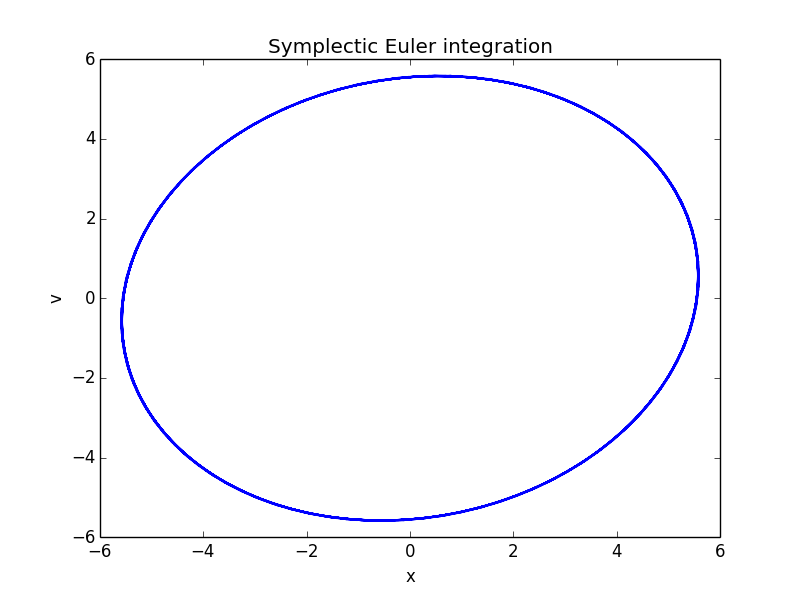
\includegraphics[height=7cm]{symplecticEuler_Sling}}
\caption{A solution to the harmonic oscillator numerically integrated with the Symplectic Euler
  Method starting from $x_{0}=5$ and $v_{0}=3$ with a stepsize of $h=0.2$. The pendulum returns to
  its original position after a full period, as it is supposed to. There is however an asymmetry in
  the solution, the pendulum reaches its highest point just after the velocity is zero, not at the
  same time. This can be fixed by using either a smaller stepsize or using a higher order
  integrator.}
\label{fig:symplectic}
\end{figure}

\subsection{Leapfrog}
\label{sec:leapfrog}
The \textit{Leapfrog} integrator is a second order integration scheme. \cite{leapfrog} That makes
its global truncation error proportional to $h^2$ (note that this is smaller than $h$ for $h<0$).
Furthermore this integrator is time reversible: if you would replace the stepsize $h$ by $-h$, you
would get back precisely the starting conditions (up to rounding error). Time reversibility thus
guarantees conservation of energy.

\begin{figure}
\center{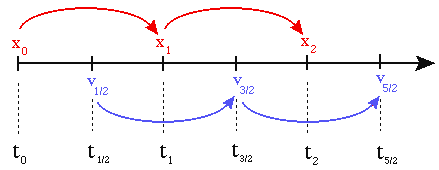
\includegraphics[height=4cm]{leapfrog}}
\caption{An illustration of the leapfrog integration scheme. The velocity starts off at half a
  timestep and the integration continues with the subsequent iterations ``leaping'' over each
  other's time.}
\label{fig:leapfrog}
\end{figure}

In figure \ref{fig:leapfrog} we see an illustration of the leapfrog integration scheme. The major
difference with the previous methods is that the leapfrog integrator is not synchronous. The
velocities and positions are calculated at different times. The integrator starts off at $x_{0}$ and
$v_{1/2}$ after which they take full steps leaping over each other's time. In practice we don't have
the initial velocity at half a timestep, so we have to kickoff the leapfrog integrator by doing half
an integration step of the velocity using another integrator, for example using the Forward Euler
Method:
\begin{minted}[]{python}
vHalf[0] = v0 + 0.5 * h * a[0]
\end{minted}
Then the positions and velocities can leap over each other:
\begin{minted}[]{python}
x[n + 1] = x[n] + h * vHalf[n]
vHalf[n + 1] = vHalf[n] + * h * a[n + 1]
\end{minted}
Notice that here the velocity is calculated with the new position, while in the symplectic Euler
method the position is calculated with the new velocity.

This reduction in error also further improves the performance on the harmonic oscillator. In figure
\ref{fig:leap} we see the simple pendulum now solved with the Leapfrog integrator. The difference
with figure \ref{fig:symplectic} is in the general shape, it is now symmetric in the x and y axes
instead of being a slanted ellipse. This is due to the Leapfrog integrator being of higher order.

\begin{figure}
\center{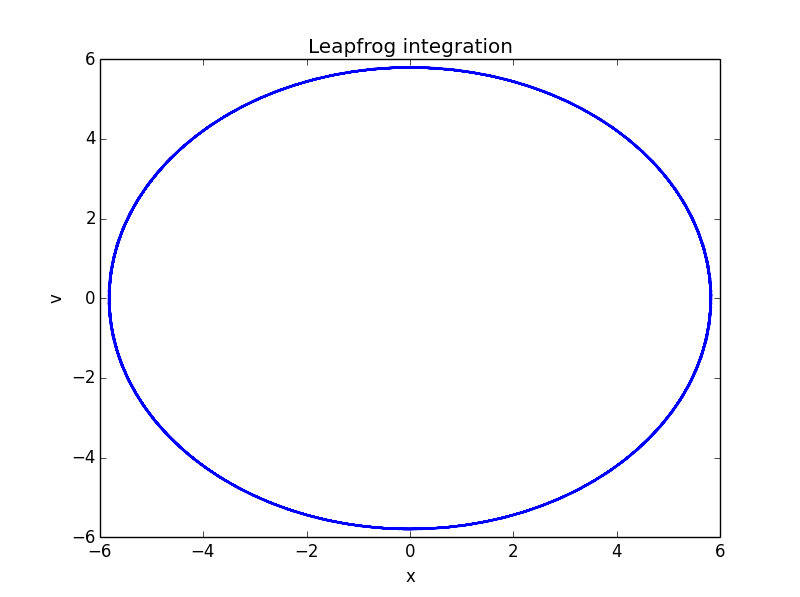
\includegraphics[height=7cm]{Leapfrog_Sling}}
\caption{A solution to the harmonic oscillator numerically integrated with the Leapfrog integrator
  starting from $x_{0}=5$ and $v_{0}=3$ with a stepsize of $h=0.2$. The pendulum returns to its
  original position after a full period, .}
\label{fig:leap}
\end{figure}

We've now seen three methods, each improving over the previous one. Our last method is of second
order and conserves the energy in the sytem. An important observation to keep in mind is that these
methods all require about the same number of floating-point operations. The Leapfrog scheme is
computationally as intensive as the Forward Euler Method but is still of a higher order. We could
look at integrators of higher order, but they will require more flops. Thus we consider the Leapfrog
integrator as most fitting for our purposes: fast, energy conserving and of second order.

\section{Implementation}
We've studied the necessary mathematics and algorithms to implement the few body problem. We've
implemented these in JavaScript so aspiring gravity simulators only need a web browser with internet
access. Our implementation is called Sunsistemo, available on \url{https://sunsistemo.js.org}. The
source code is available at \url{https://github.com/sunsistemo/sunsistemo}.

We made use of the JavaScript library three.js which enables users to make GPU accelerated 3D
graphics in the browser through the use of WebGL. WebGL in itself is cumbersome to use as it is a
low level language. A simple 3D object would require many lines of control and shader code, however
three.js offers an higher level API for the creation and manipulation of 3D objects which are then
rendered using WebGL.

In figure \ref{fig:flowchart} the flowchart of Sunsistemo is shown, a high level overview of
Sunsistemo's design. We can divide Sunsistemo in two parts, simulation and visualization. Body
objects with positions and velocities live in the simulation part and they are represented by
three.js spheres in the visualization part.

\begin{figure}
\center{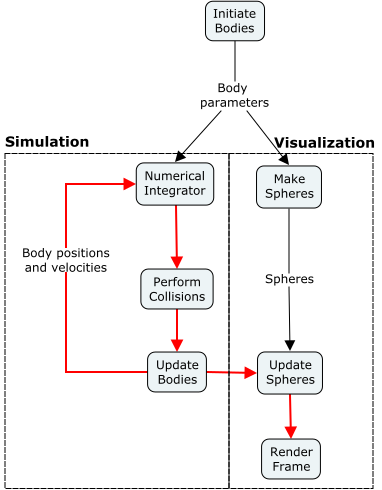
\includegraphics[height=9cm]{Flowchart}}
\caption{Highlevel flowchart of Sunsistemo. Red arrows represent the processes that are executed
  every frame of the visualization}
\label{fig:flowchart}
\end{figure}


\subsection{Simulation}
The simulation starts with initiation of a system containing an array of body objects. Body objects
have some static parameters (mass, radius, texture, rotation) and some dynamic variables (position,
velocity) which can be changed during the simulation. The system also defines some simulation and
visualization parameters (stepsize, steps per animation frame, etc.). Every timestep new body
positions and velocities are calculated from the values of the previous timestep using the leapfrog
algorithm from section \ref{sec:leapfrog}. After every step, each body is checked for collisions
which are performed using the algorithm described in section \ref{sec:collisions}. The integration
and collision algorithms update the velocity and position vectors of each body so these new
variables can be used to update the visualization and are used as input for the next simulation
step.

\subsection{Systems}
Sunsistemo is built in a modular fashion so it can simulate many different systems. The systems
currently defined are:
\begin{itemize}
\item \textbf{Two Bodies:} two bodies in a Keplerian orbit.
\item \textbf{Three Bodies:} two planets orbiting a star. This system isn't stable, after some time
  one of the planets leaves.
\item \textbf{The Solar System:} the Sun, Mercury, Venus, Earth, the Moon, Mars, Jupiter, Saturn,
  Uranus, Neptune and Pluto. The initial conditions for this system are from NASA's HORIZONS system.
  \cite{stan}
\item \textbf{Random bodies:} a collection of many bodies each with random positions and velocity.
\item \textbf{Angular Momentum:} many planets orbiting around the Sun. There is no interaction when
  bodies collide: they pass through each other.
\item \textbf{Angular with Bounce:} same as the previous but now the planets are balls and they
  experience elastic collisions when they touch.
\item \textbf{N-body choreographies:} there are some analytic solutions for the N-body problem where
  $n>2$. These are special cases where often the bodies are of equal mass. We've implemented all
  systems reported in the paper by {{\v S}uvakov} and {Dmitra{\v s}inovi{\'c}}.
  \cite{three-body-planar} These systems are in theory stable, but in our simulation the numerical
  errors build up and some bodies escape.
\end{itemize}

\subsection{Visualization}
The initial idea of the project was to make a visualization of the few-body problem that is
appealing to the eye and pleasant to use. Using three.js the following features were added to make
the visualization aesthetically attractive:
\begin{itemize}
\item \emph{Spheres}\\
  To add to the visual experience of the end user, instead of point particles the visualization uses
  sphere geometries of variable size to visualize the bodies. This decision made it necessary to
  implement close range interaction, as described in chapter \ref{sec:collisions}, as the spheres
  would pass through each others radius without it. Sphere size can be coupled to the body radius,
  for example to show the relative physical size of the planets in the solar system. The number of
  polygons of which the sphere is build up can be adapted to alleviate the computational cost in
  case of systems with many bodies. After each simulation cycle the new body position values are
  used to update sphere positions and the new simulation frame is rendered.

\item \emph{Lighting}\\
  To achieve better 3D experience, proper lighting is necessary. A combination of ambient lighting
  and a point source is used. In the solar system the point source can be coupled to the sphere
  representing the sun. To the sun we've also added a halo sprite around the sphere, which mimics
  the solar atmosphere. Phong shading is used to determine the light level on the geometries. Phong
  shading interpolates the surface normals across a geometry to show a smoother surface, in contrast
  to flat shading which calculates the light level from the actual polygon surface normal.


\item \emph{Textures}\\
  For visual appeal and to be able to discern the different bodies, a body texture is applied to the
  sphere geometries. Textures of the eight solar system planets, the Sun and Pluto were used for the
  solar system and other random systems. \cite{planettexture} Different textures can be used to
  mimic other physical systems, for example the random bodies system where softball and tennisball
  textures are used. \cite{balltexture}

\item \emph{Bumpmap}\\
  The use of the point light source, which causes directed lighting, enables us to assign a bump map
  to the spheres. The bump map adjusts the surface normals which are used for calculating the
  surface lighting. There is no use in this for simulation purposes but from an aesthetic point of
  view it is interesting to have a detailed surface instead of a smooth one. Since we already use
  Phong shading, the implementation of a bump map does not require much more computational power.
  For even more realistic lighting a specular map can be added which adjusts the amount of specular
  reflection as opposed to diffuse reflection. For example, the water covered parts of the earth
  surface have a higher specular reflection while the reflection of land covered parts is mainly
  diffuse. Bump and specular maps where obtained from the same source as body textures.


\item \emph{Scaling}\\
  To make an appealing visualization of the solar system it is inevitable to scale the objects radii
  with respect to the orbit radii. Without this scaling the ratio of orbit radius to object radius
  for the earth would be:
\begin{equation}
q = \frac{1.5 *10^{11} \mbox{ m}}{6.4*10^6 \mbox{ m}} = 2.3 *10^4
\end{equation}
Consequently we would need a screen of approximately $10^4$ pixels wide to see its full orbit and
have the earth visualized as a single pixel. Additionally the ratio between the radius of the Sun
and the radius of the inner planets is in the order of $10^2$ and $10^1$ for the radii of inner and
outer planets. This implies we need a non-linear scaling for the size of the celestial objects. We
decided on a scaling of:
\begin{equation}
s = \sqrt[5]{r_{\mbox{planet}}} \cdot 2 \cdot 10^9
\end{equation}

This scaling works as an equalizer for the object radii because of the fifth root and blows up the
size of the objects to be of approximately the same order as the orbit radius.

\item \emph{GUI}\\
  To let users access and interact with the visualization from the browser a graphical user
  interface is needed. While this may change in the future, for now a simple button menu was chosen
  which lets the user select predefined systems and choreographies of which one is the solar system.
  The interface was built with the Javascript data binding library D3.js. \cite{d3lib}

\item \emph{Interaction}\\
  Users can also interact in real-time with the simulation. Using their mouse they can manipulate
  the camera: left-clicking and dragging will change the perspective of the camera, right-clicking
  and dragging will change the position of the camera and scrolling will zoom in or out.

\end{itemize}


\section{Validation}
We've created a model of gravity using Newton and the Leapfrog integrator. Everyone can create a
model, but few can create a good model. That is why it's required to validate the model. We will
perform an error analysis for the solar system simulation.

We can define the error of the simulation at time $t$ as:
\begin{equation} \label{eq:error}
E = \frac{1}{n} \sqrt{ \sum_{i=0}^{n} \|\hat{\vect{x}}_i - \vect{x}_i\|^2},
\end{equation}
where $n$ is the number of bodies, $\hat{\vect{x}}_i$ the computed position of body $i$ and
$\vect{x}_i$ its real position. A validation of the model would then look like a plot of the error
as defined in equation \ref{eq:error} over time.

\subsection{The Solar System} 
The solar system is constantly being observed by astronomers. NASA's HORIZONS system provides highly
accurate data for objects in the solar system. They report having data on ``(696540 asteroids, 3366
comets, 178 planetary satellites, 8 planets, the Sun, L1, L2, select spacecraft, and system
barycenters)'' \cite{stan} We took the initial conditions for the solar system from NASA for the
simulation. For the validation we compare the computed data with data from NASA over a range of
years

In figure \ref{fig:err_leap} we see the error of the leapfrog method with stepsizes of 24 hours
(blue) and 12 hours (green). The error increases linearly over time. Lowering the stepsize naturally
decreases the error. The red line has errors with exactly half of those of stepsize 24h. For a
second order integrator halving the stepsize should lead to a $2^2$ factor of decrease in error, but
this was not observed. The distance between the red and green lines show that halving the stepsize
roughly also halves the error.
\begin{figure}
\center{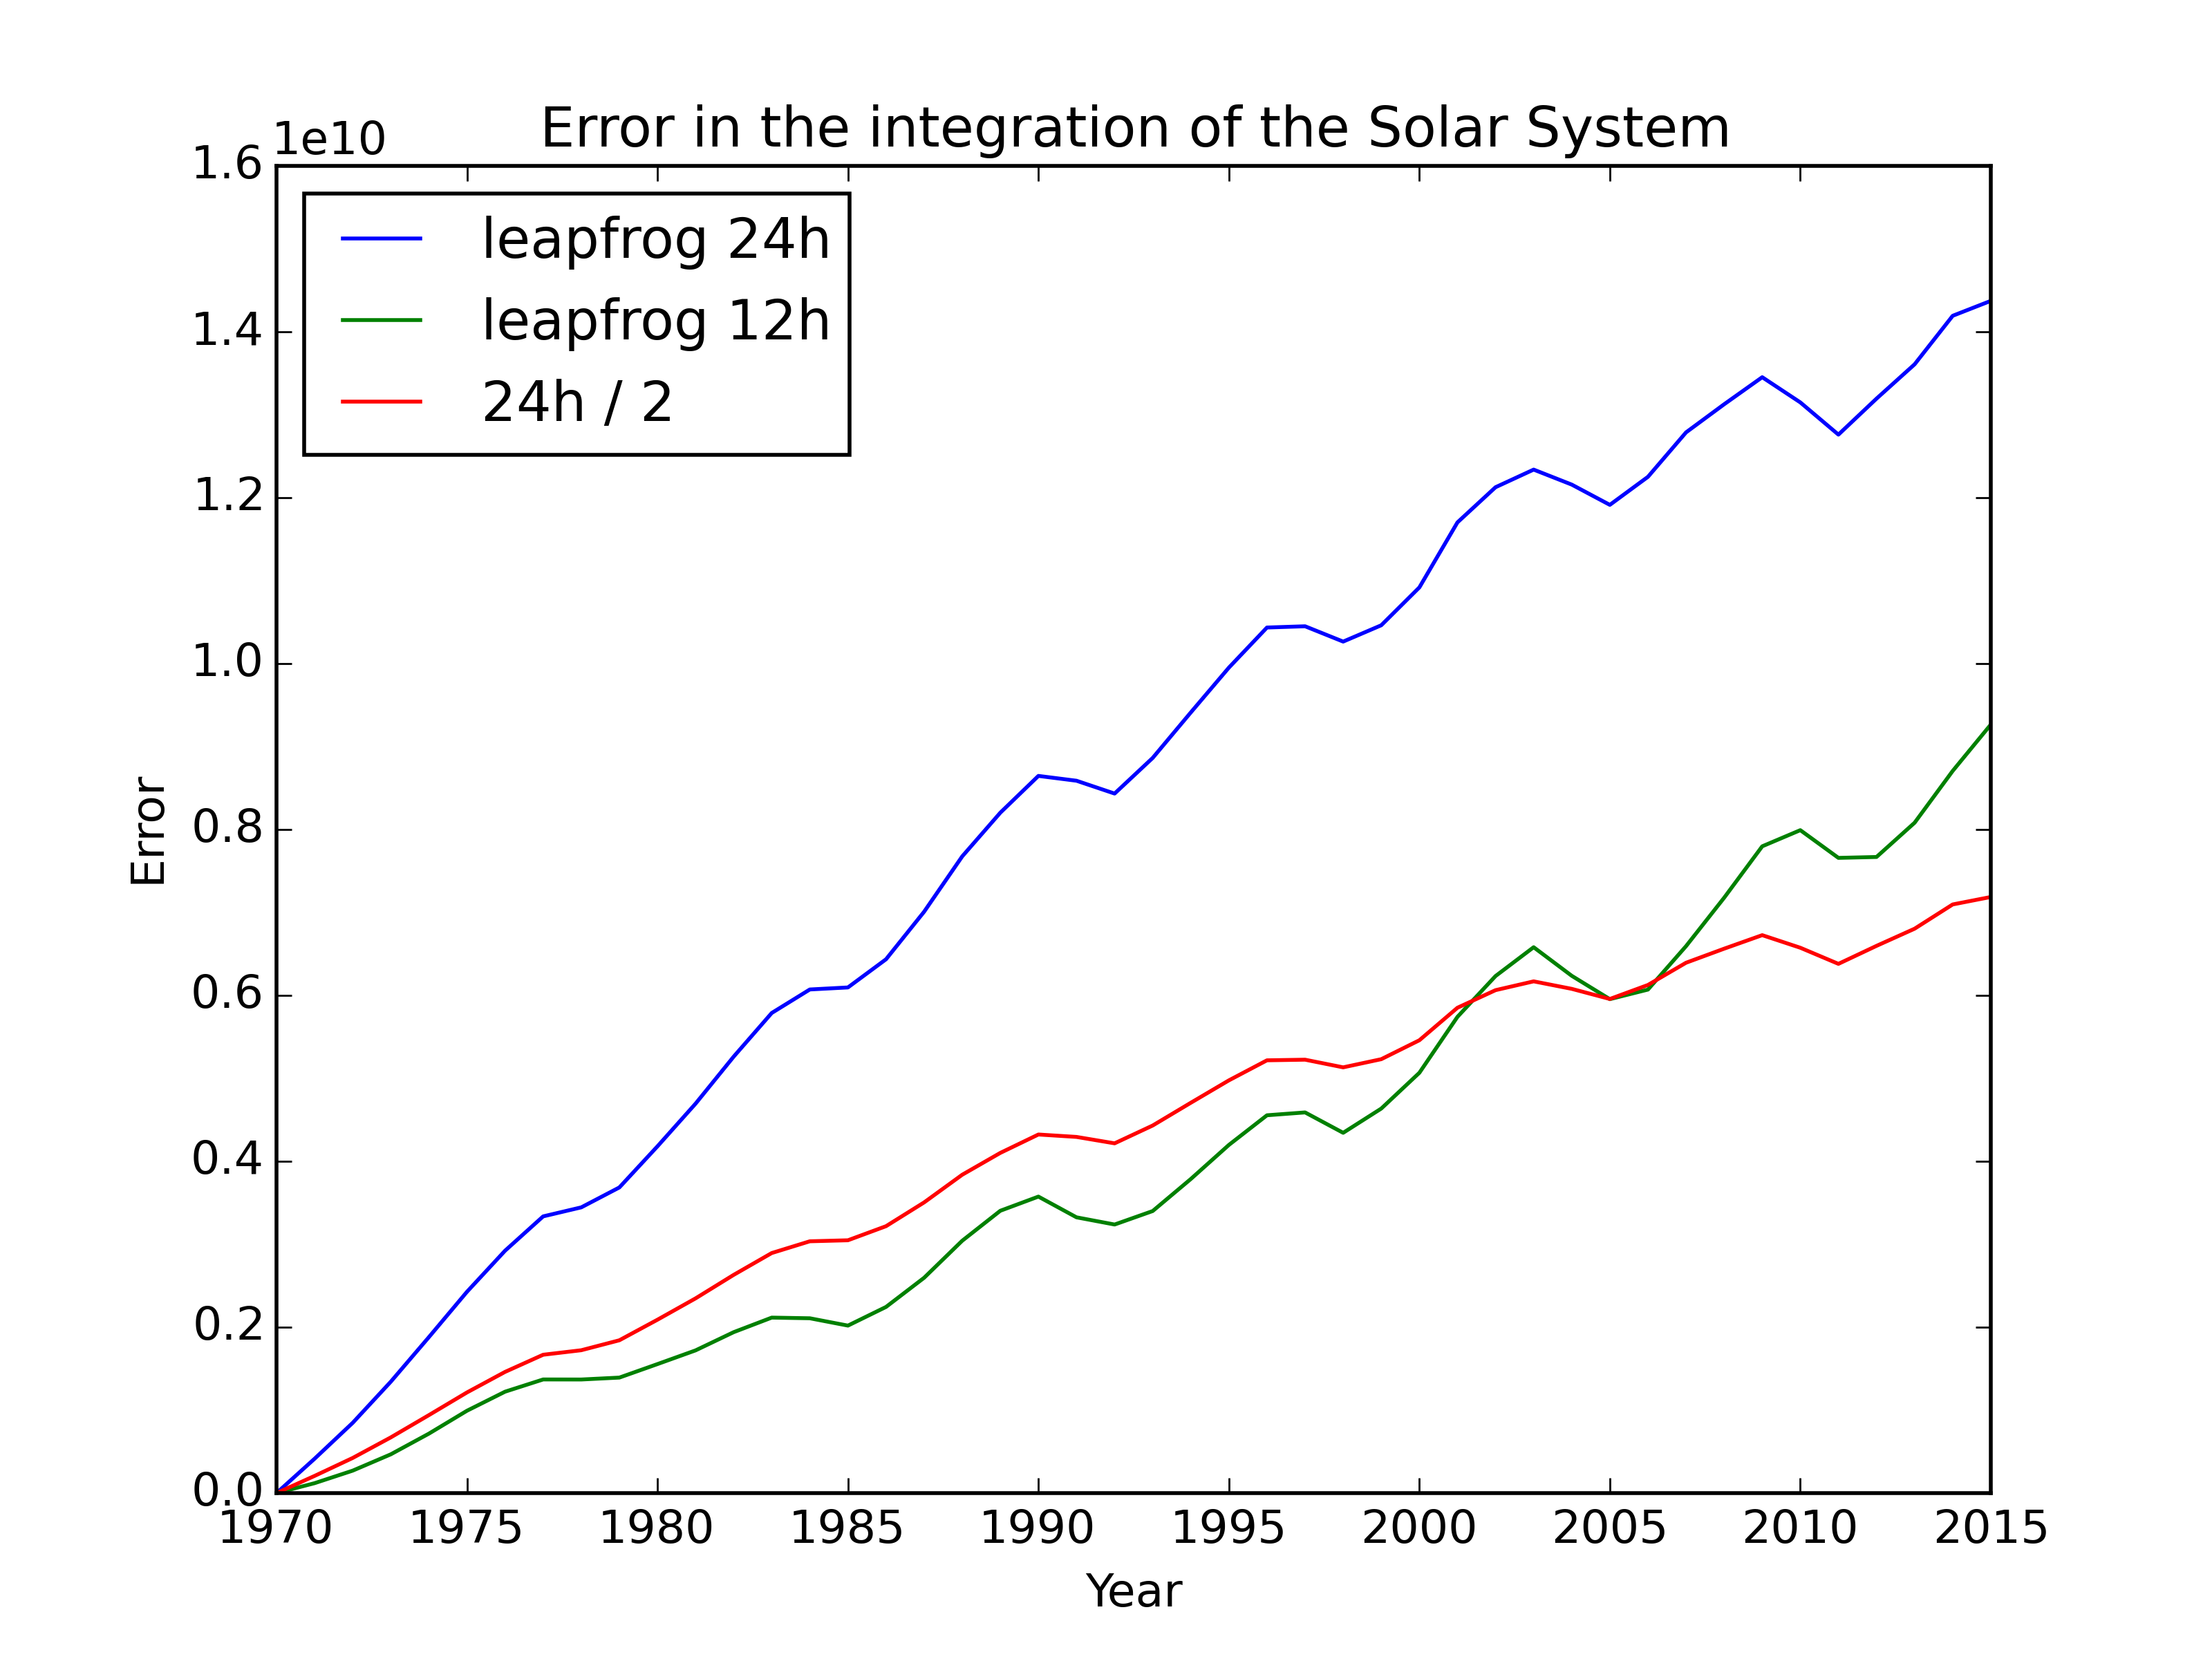
\includegraphics[height=9cm]{errors_leapfrog}}
\caption{The error over a range of years in the integration of the Solar System using the Leapfrog
  integration method.}
\label{fig:err_leap}
\end{figure}

In figure \ref{fig:err_symp} we see the performance of the symplectic Euler method. There is a clear
difference in how the error evolves: it is periodic instead of linear. Another clear difference is
in the effectiveness of reducing the error in decreasing the stepsize: halving gives an error of
roughly the same magnitude. This is expected as the leapfrog integrator was of higher order.
\begin{figure}
\center{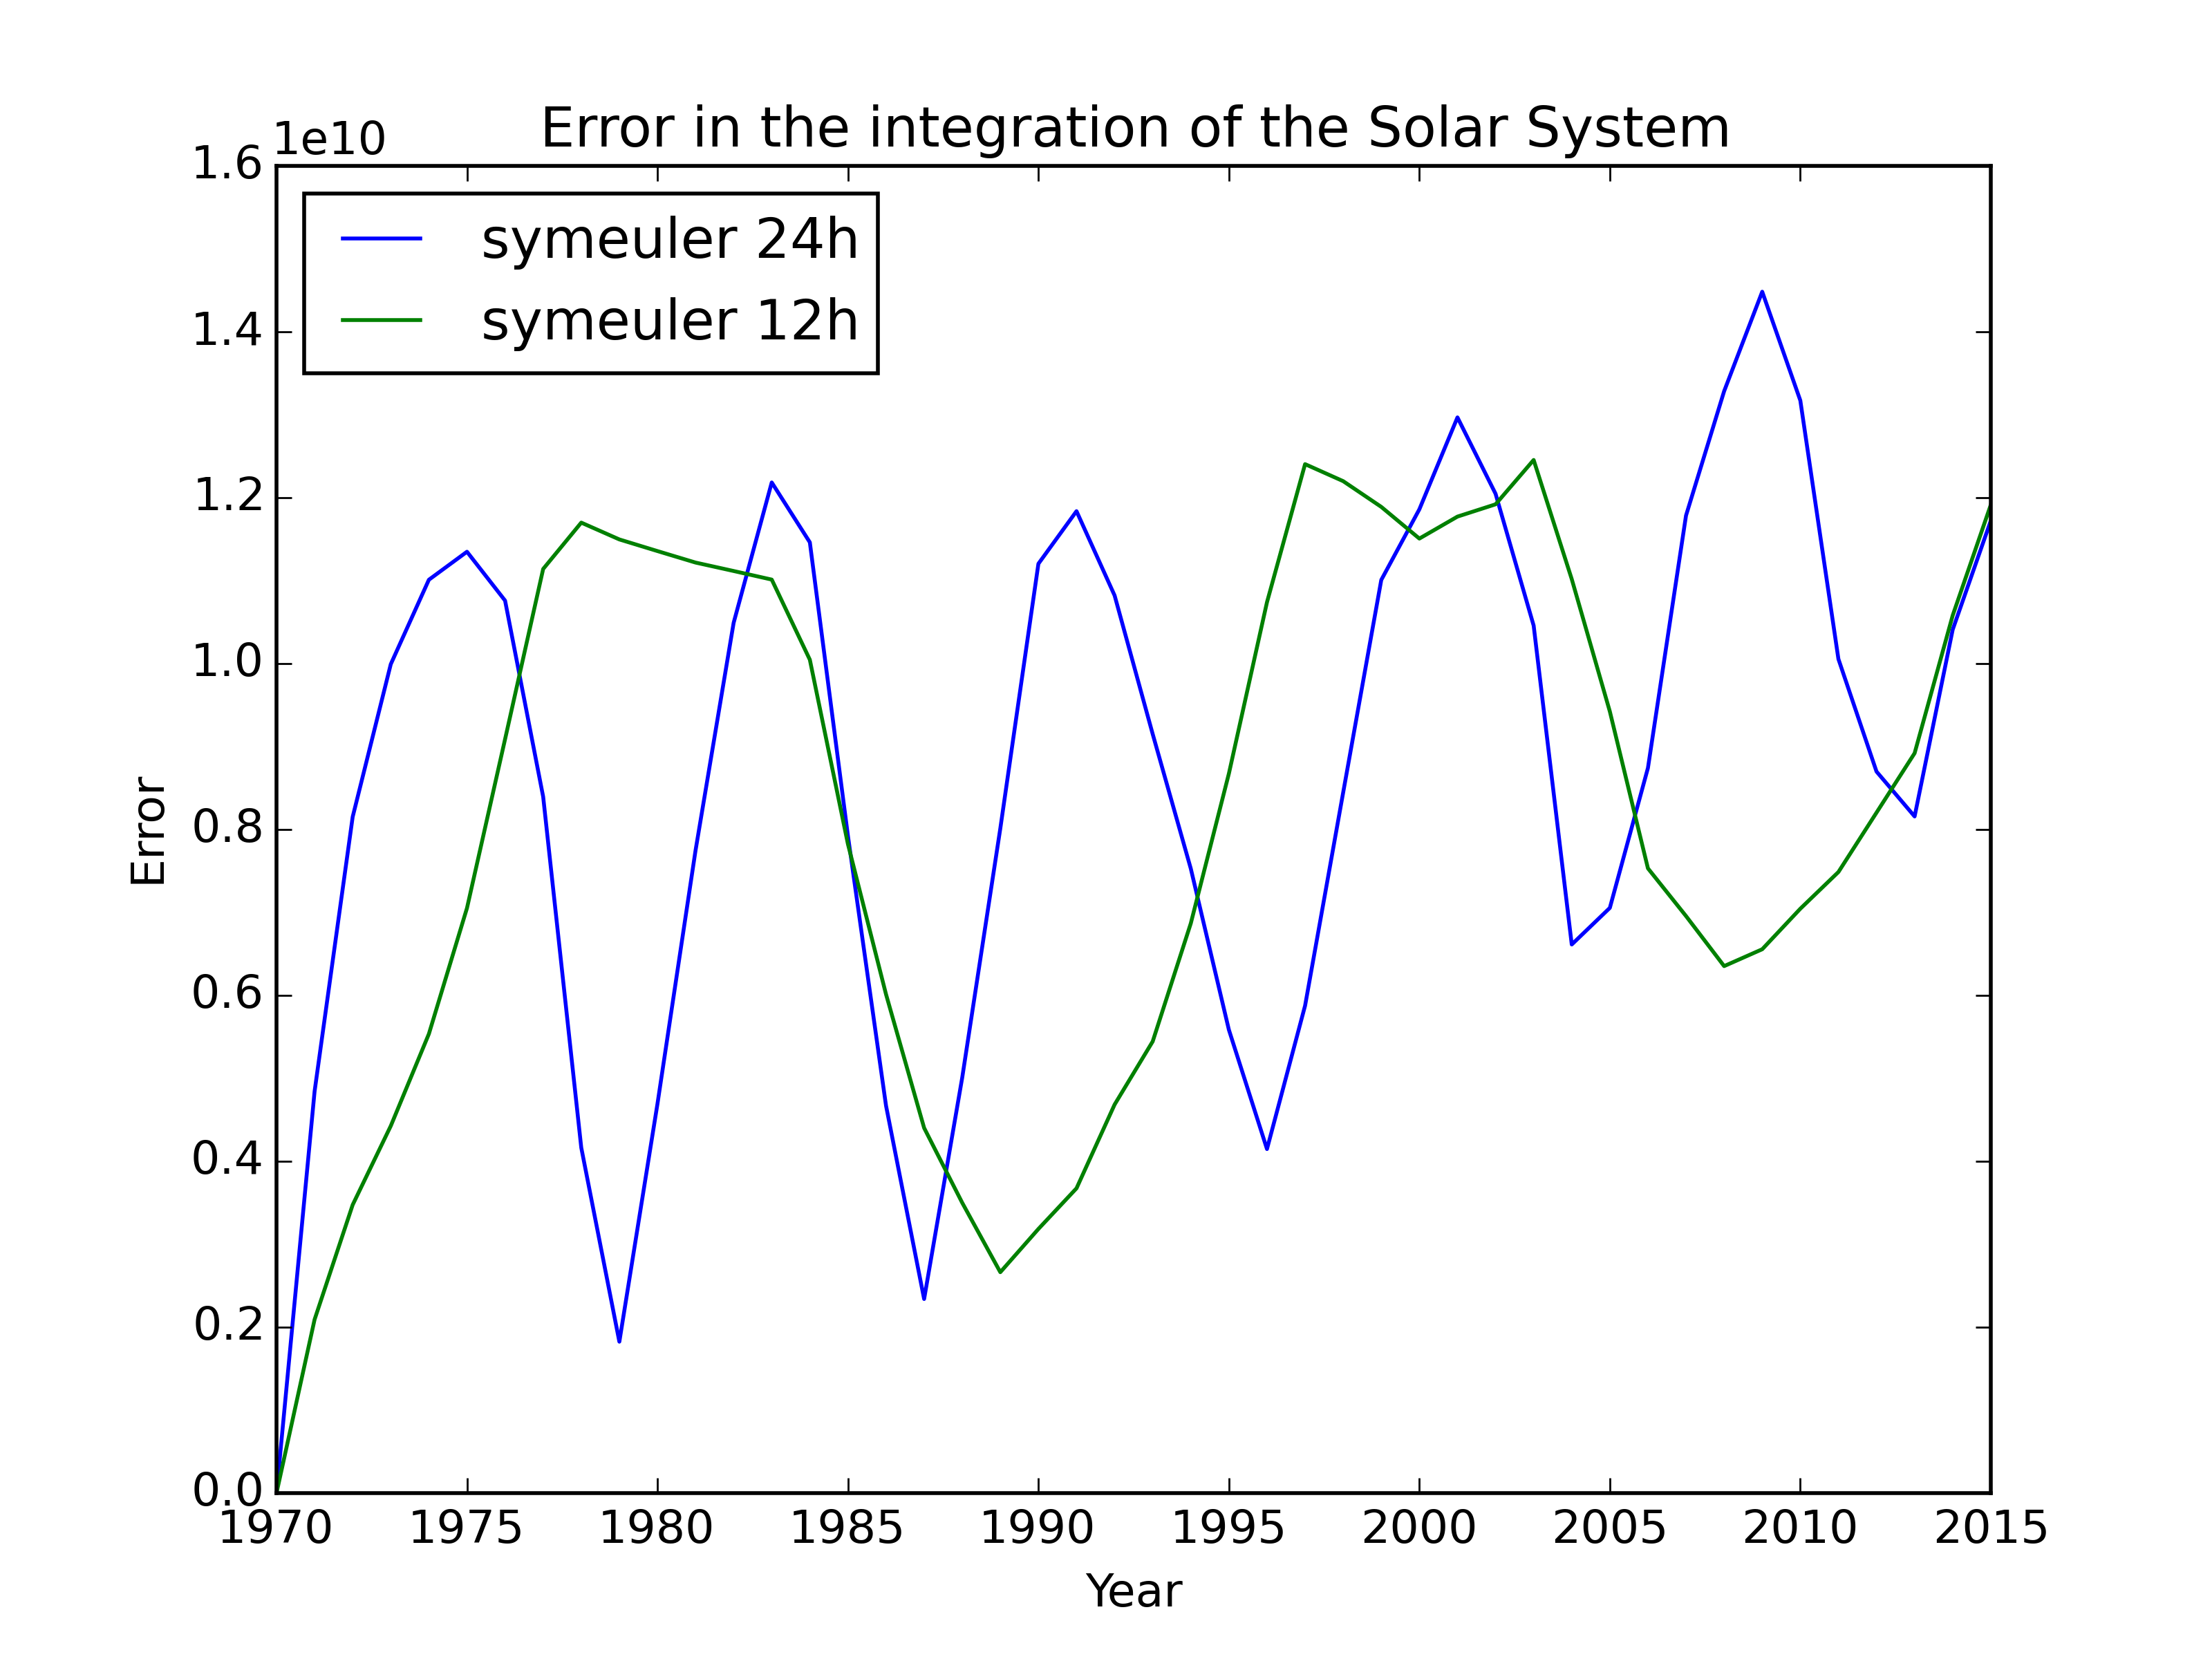
\includegraphics[height=9cm]{errors_symplectic1}}
\caption{The error over a range of years in the integration of the Solar System using the Symplectic
  Euler integration method.}
\label{fig:err_symp}
\end{figure}

Finally in figure \ref{fig:err_leap_sym} we see a comparison between performance of the leapfrog and
symplectic Euler method. This is clear evidence confirming that the Leapfrog integrator has an
overall smaller error than the Symplectic Euler method.
\begin{figure}
\center{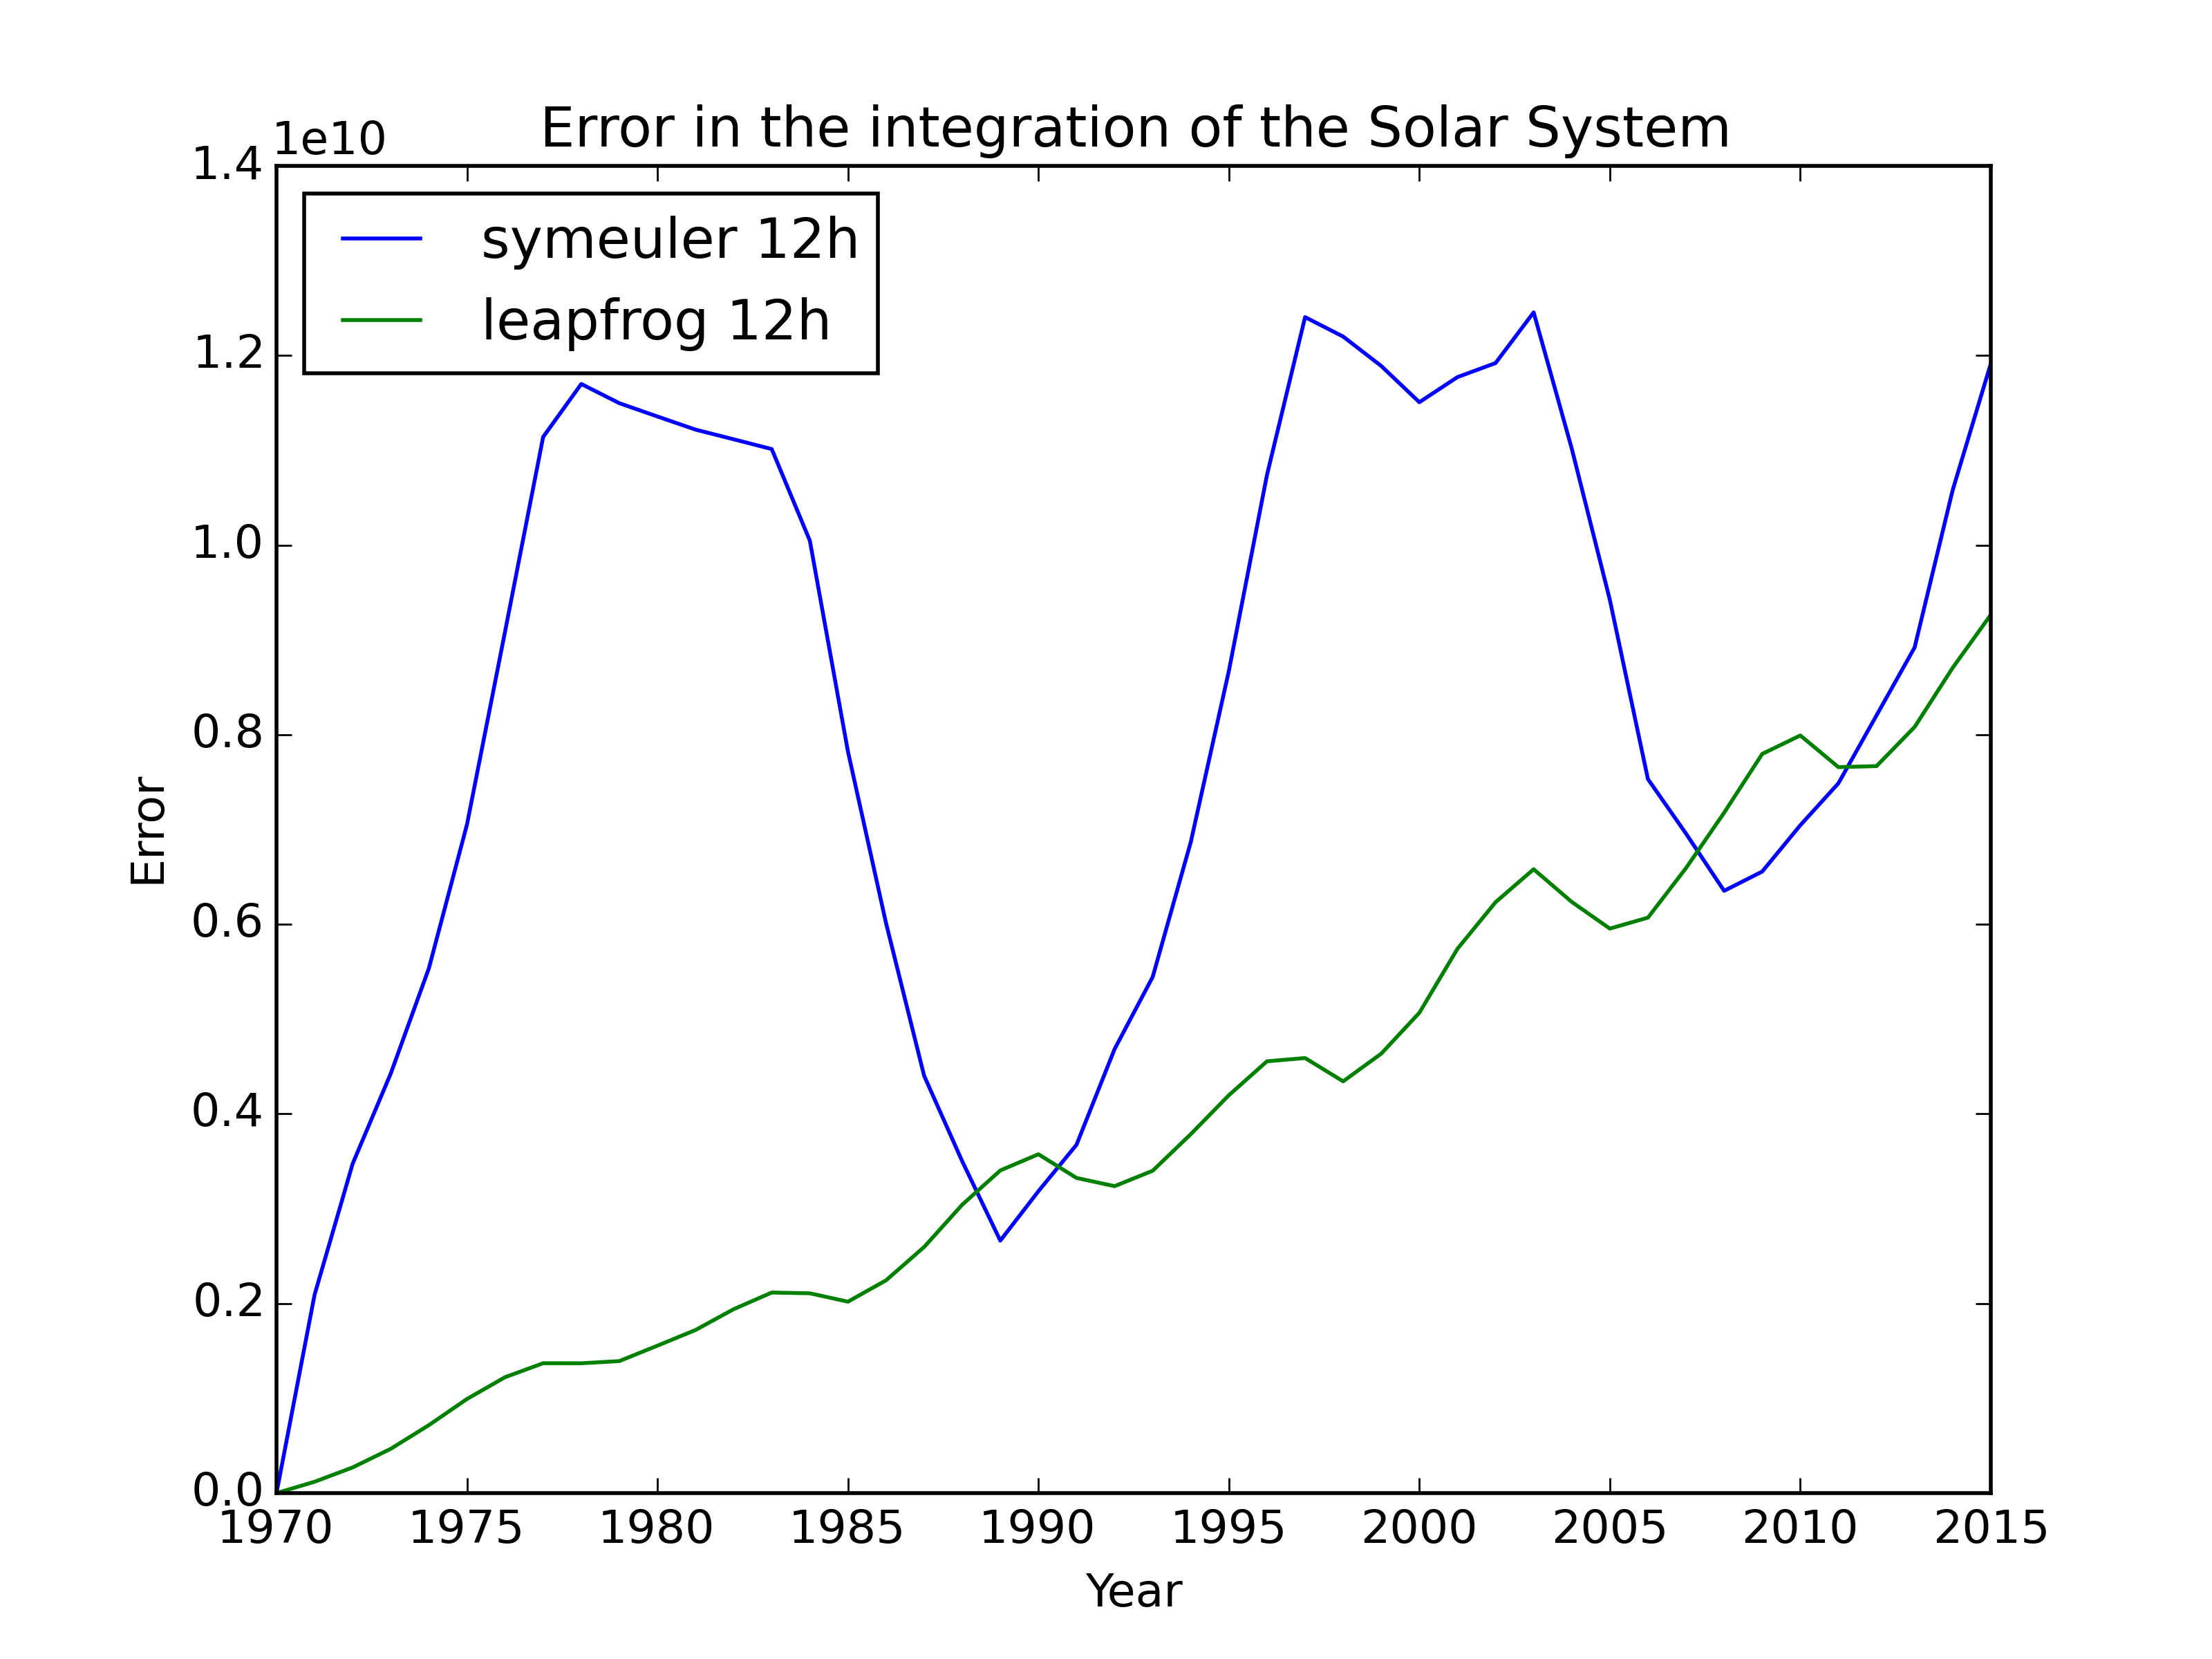
\includegraphics[height=9cm]{errors_leap_symplectic}}
\caption{The error over time for the Leapfrog and Symplectic Euler methods. The Leapfrog method
  performs better with the same stepsize.}
\label{fig:err_leap_sym}
\end{figure}

This concludes the validation. Of course we can decrease the stepsize to get lower and lower errors
but that is not the point of the validation. We've confirmed that:
\begin{enumerate}
\item The simulation ``works''. The magnitude of the error is sensible, it is on the order of the
  position of Mercury (1E10). The gradual increase in error is also as expected.
\item We've demonstrated that the Leapfrog method does indeed have smaller errors than the
  Symplectic Euler method.
\end{enumerate}

\section{Conclusions}
% In this section you give a clear resume of the conclusions from your work and discuss its relation to previous research.
% –For that reason, some authors will actually put the section on related work after the core section(s)
% –The conclusions should reflect back on the original problem statement in your introduction.
% •When applicable, your work may result in suggestions on how to further validate or extend your research.
We set out to make a few body simulator that is both accessible and visually pleasing. We started
with an overview of the physics and continued with numerical integration. Introducing our
implementation, Sunsistemo \cite{sunsistemo}, we discussed the visualization techniques that were
applied to make it appealing. We have also validated the numerical model and shown that the choice
for implementing the Leapfrog integrator was not in vain. In figure \ref{fig:sunsistemoPrtSc} we see
a screenshot of Sunsistemo that can be reproduced by anyone within seconds by going to the website.
With that we conclude that we've largely accomplished our initial goals.

This is however not the end, there are still many aspects of the model that can be improved.

\begin{figure}
\center{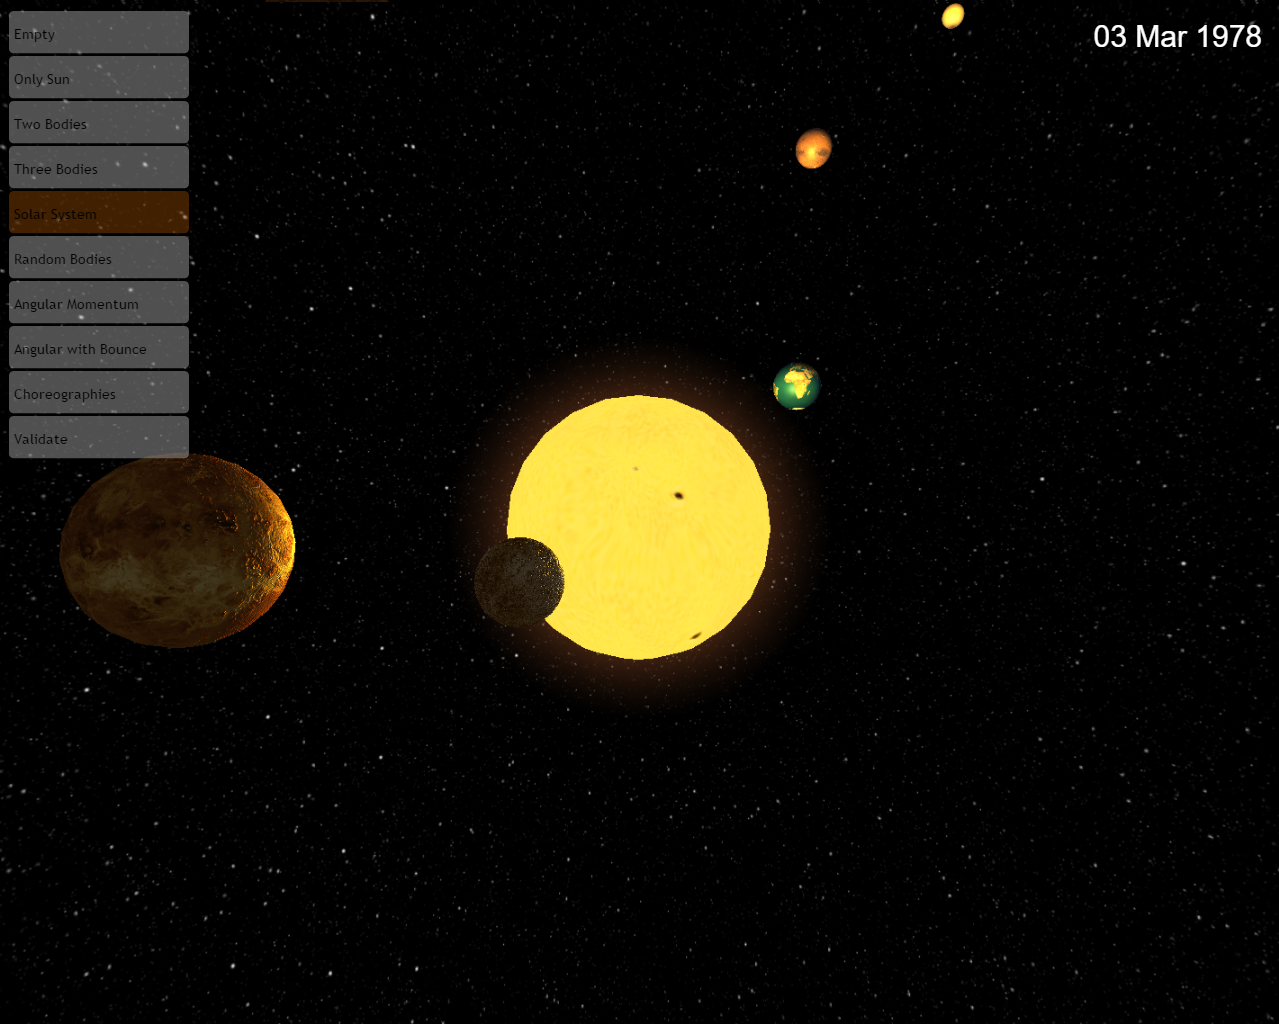
\includegraphics[height=9cm]{sunsistemoPrtSc}}
\caption{A screenshot of Sunsistemo in action. Seen are the Sun and its five inner planets orbiting
  around it.}
\label{fig:sunsistemoPrtSc}
\end{figure}

\section{Recommendations}
In further development of Sunsistemo much can be done to improve the application. Both on the
simulation side and on the graphical visualization side. These major improvements are more or less
ordered by priority and can also be found on the GitHub page \cite{sunsistemoGH} amongst other minor
issues.

\begin{itemize}
\item \emph{Adaptive stepsize}\\
  The closer two bodies approach each other, the higher the gravitational acceleration. With a
  faster changing velocity, the error in the simulation also grows because the linear distance
  covered per step becomes bigger. In Sunsistemo this can most prominently be seen when collisions
  are turned off, bodies approach each other to very small distance and tend to fly out of orbit
  after these close approaches because they maintain the high velocities obtained at perihelion for
  too long due to a large step size. A solution would be to change the step size to the order where
  this effect does not occur, however this would cost a lot of computational power and is not
  necessary for most part of the orbit since acceleration and velocities are not that large. A
  variable step size, proportional to the minimum separation between the body and any other body,
  could solve this problem.

\item \emph{DIY simulations}\\
  The goal of Sunsistemo was to encourage people to start experimenting with the n-body simulator,
  at the moment however the interaction with the end user is limited to the simple GUI which only
  offers a wide range of predefined systems. It would be better if users could define their own
  system by selecting the amount of bodies and whether they are distributed randomly or at specified
  initial positions and velocities. The API of Sunsistemo is suitable for this, but the GUI still
  has to be build.

\item \emph{Validation with the analytical 2-body problem}\\
  Besides the validation using NASA data of the solar system there is another way validating the
  model using the analytic solution of the 2-body problem. The differential equation for a system of
  two bodies of mass $m_1$ and $m_2$:
\begin{equation}
\label{eq:dtTwoBody}
\frac{dr}{dt} = \sqrt{\frac{2}{\mu}}\left(E-\frac{1}{2}\frac{L^2}{\mu r^2} + \frac{G m_1 m_2}{r}\right)^{\frac{1}{2}}
\end{equation}

with $\mu = \frac{m_1 m_2}{m_1 + m_2}$ the reduced mass and $r = |{\vect{r}_1 - \vect{r}_2}|$ the
distance between the two bodies. It could be integrated directly, however no explicit solution for
$r(t)$ can be obtained. So a different approach should be used converting the Cartesian simulation
coordinates to cylindrical reduced mass coordinates and compare them with solutions of the form
$r(\theta)$ which can be obtained.


\item \emph{Higher order (symplectic) integrators}\\
  The currently used leapfrog algorithm is a second-order symplectic integrator. To achieve a more
  stable simulation we can implement integration algorithms of higher order. This will result in
  smaller errors, however higher order integrators in general require more function evaluations per
  simulation step. Nevertheless it would be interesting to test several integrators like Verlet
  integration or the Runge-Kutta method.

\item \emph{Approximation scheme}\\
  When using these higher order integrators it might be necessary to implement a more sophisticated
  algorithm to add all interactions on a body and approximate this for far away bodies to decrease
  computational cost. For example the Barnes-Hut method which divides space in cubic cells and lets
  the body of interest interact with the center of mass of each cell instead of every single body.
  This would also possibly allow Sunsistemo to scale up to be an n-body simulator instead of the
  few-body simulator it is now with decreasing performance at around 400 bodies.

\item \emph{Better physics for collisions}\\
  At the moment the physics of collisions between bodies is described by the perfect elastic
  collision. Perfect elastic collisions do not exist in nature, so to improve the model the close
  range interaction should be changed. Merging is an interesting option for a colliding planet and
  star or black hole, semi-elastic collisions could also be implemented for smaller celestial
  objects, which bounce off each other but lose energy in the process. It must be said however that
  for simulation of systems like the solar system, collisions are not of importance because of the
  difference in scale between orbit and object radii.

\item \emph{Stereoscopy}\\
  To make the visualization even more appealing the 3D vision could be enhanced by adding
  stereoscopy. This is easy to implement by rendering the same simulation from two different angles
  and overlay the rendered frames with different hue filters for anaglyph or stack them side-by-side
  for display on a 3D television, projector or oculus rift.
\end{itemize}


\bibliography{references}
\bibliographystyle{unsrt}

\end{document}
